% fancytikzposter.tex, version 2.1
% Original template created by Elena Botoeva [botoeva@inf.unibz.it], June 2012
% 
% This file is distributed under the Creative Commons Attribution-NonCommercial 2.0
% Generic (CC BY-NC 2.0) license
% http://creativecommons.org/licenses/by-nc/2.0/ 


\documentclass{a0poster}

\usepackage{fancytikzposter} 


%%%%%%%%%%%%%%%CUSTOM HEADER
\renewcommand{\Re}{\operatorname{Re}}
\renewcommand{\Im}{\operatorname{Im}}
\usepackage{braket}
\newcommand{\mean}[1]{\langle #1 \rangle}
\usepackage{titlesec}
\titlespacing\section{0pt}{12pt plus 0pt minus 0pt}{0pt plus 0pt minus 0pt}
\usepackage{graphicx}
\bibliographystyle{plain} %apsrev4-1}
%%%%%%%%%%%%%%%%%%%%%%%%%%%%%%


%%%%% --------- Change here if you want ---------- %%%%%
%% margin for the geometry package, must be changed before using the geometry package
%% default value is 4cm
\setmargin{0.8}

%% the space between the blocks
%% default value is 2cm
\setblockspacing{0.45}

%% the height of the title stripe in block nodes, decrease it to save space
%% default value is 3cm
% \setblocktitleheight{3}

%% the number of columns in the poster, possible values 2,3
%% default value is 2
\setcolumnnumber{3}

%% the space between two or more groups of authors from different institutions
%% used in \maketitle
% \setinstituteshift{10}

%% which template to use
%% N1 simple, standard look, with a colored background and gray boxes
%% N2 board with nodes
%% N3 another standard look
%% N4 envelope-like look
%% N5 with a wave-like head, original idea taken from
%%%% http://fc09.deviantart.net/fs71/f/2010/322/1/1/scientific_poster_by_nabuy-d333ria.jpg
\usetemplate{2}

%% components of the templates
%% (the maximal possible numbers are mentioned as the parameters)
% \usecolortemplate{4}
% \usebackgroundtemplate{5}
% \usetitletemplate{2}
% \useblocknodetemplate{5}
% \useplainblocktemplate{4}
% \useinnerblocktemplate{2}


%% the height of the head drawing on top 
%% applicable to templates N3, 4 and 5
% \setheaddrawingheight{14}


%% change the basic colors
%\definecolor{myblue}{HTML}{008888} 
%\setfirstcolor{myblue}% default 116699
%\setsecondcolor{gray!80!}% default CCCCCC
%\setthirdcolor{red!80!black}% default 991111

%% change the more specific colors
% \setbackgrounddarkcolor{colorone!70!black}
% \setbackgroundlightcolor{colorone!70!}
% \settitletextcolor{textcolor}
% \settitlefillcolor{white}
% \settitledrawcolor{colortwo}
% \setblocktextcolor{textcolor}
% \setblockfillcolor{white}
% \setblocktitletextcolor{colorone}
% \setblocktitlefillcolor{colortwo} %the color of the border
% \setplainblocktextcolor{textcolor}
% \setplainblockfillcolor{colorthree!40!}
% \setplainblocktitletextcolor{textcolor}
% \setplainblocktitlefillcolor{colorthree!60!}
% \setinnerblocktextcolor{textcolor}
% \setinnerblockfillcolor{white}
% \setinnerblocktitletextcolor{white}
% \setinnerblocktitlefillcolor{colorthree}




%%% size of the document and the margins
%% A0
% \usepackage[margin=\margin cm, paperwidth=118.9cm, paperheight=84.1cm]{geometry} 
\usepackage[margin=\margin cm, paperwidth=84.1cm, paperheight=118.9cm]{geometry}
%% B1
% \usepackage[margin=\margin cm, paperwidth=70cm, paperheight=100cm]{geometry}



%% changing the fonts
\usepackage{cmbright}
%\usepackage[default]{cantarell}
%\usepackage{avant}
%\usepackage[math]{iwona}
\usepackage[math]{kurier}
\usepackage[T1]{fontenc}


%% add your packages here
\usepackage{hyperref}





\title{Bohmian Mechanics and Contextuality in (q,p)}
\author{Atul Singh Arora\\
  QCQI Group, IISER Mohali, India %\\
  % \texttt{ms11003@iisermohali.ac.in}
}


\begin{document}

%%%%% ---------- the background picture ---------- %%%%%
%% to change it modify the macro \BackgroundPicture
\ClearShipoutPicture
\AddToShipoutPicture{\BackgroundPicture}

\noindent % to have the picture right in the center
\begin{tikzpicture}
  \initializesizeandshifts
  % \setxshift{15}
  % \setyshift{2}


  %% the title block, #1 - shift, the default value is (0,0), #2 - width, #3 - scale
  %% the alias of the title block is `title', so we can refer to its boundaries later
  \ifthenelse{\equal{\template}{1}}{ 
    \titleblock{47}{1}
  }{
    \titleblock{47}{1.5}
  }

  %% a logo can be added to the title block
  %% #1 - anchor relative to the title block, #2 - shift, #3 - width, #3 - file name
  % \ifthenelse{\equal{\template}{2}}{ 
  %   \addlogo[south west]{(2,0)}{6cm}{unibz_b.png}
  % }{
  %   \addlogo[south west]{(2,0)}{6cm}{unibz_w.png}
  % }


  %% a block node, with the specified position (optional), title and the content
  %% #1 - where (optional), #2 - title, #3 - text
  %%%%%%%%%% ------------------------------------------ %%%%%%%%%%
  \blocknode
  {Introduction}
  {
\section*{Abstract}
    There are atleast two known theories that describe the same physical world; Quantum Mechanics and Bohmian Mechanics (also uses the Schr\"odinger Equation). While the latter is not popularly known, it provides exceptional clarity about certain aspects of reality. So far, no tests are known that can distinguish these two. One fundamental difference between them is that that the latter is deterministic (in the sense that $(q,p)$ are well defined). The purpose of this thesis is to get these theories head on; we aim to construct a theoretical situation where this type of determinism is refuted by Quantum Mechanics (using generalization of the GHZ test, contextuality etc.) and analyze it using Bohmian Mechanics. This is a step towards understanding the relation between contextuality and non-locality.
  %}

% \blocknode
%   {Abstract}
%   {The purpose of the current project will be to resolve the following apparent paradox. How can both (A) and (B) be correct, where (A) and (B) are defined as: (A) $(q,p)$ can't have predefined values to be consistent with Quantum Mechanics (QM). This can be explained by a test called ``the GHZ test''. This test claims to prove that there's no reality, viz. variables we measure can't have predefined values. This test was originally for spins. It has now been extended to $(q,p)$. (B) Bohmian Mechanics (BM) assigns $(q,p)$ precise values and has been so far shown to be consistent with all predictions of QM.\\
% This paradox has not been studied yet and it is particularly interesting for if BM is unable to predict the QM result, then we'd know at once BM is wrong. If BM does predict the QM result, we'd know that the claim made by the GHZ state, must be valid in a restricted sense.
% }

  %\blocknode
  %{Introduction}
  %{
\section*{Content}
    I will first discuss Bohmian Mechanics and then go on to discuss the known standard tests of determinism (GHZ and contextuality). Thereafter I will describe how the GHZ test is explained from the Bohmian perspective and also discuss a generalization of the GHZ test to phase space $(q,p)$. Finally, I'll show some simulation results which will be generalized in the future to perform the generalized GHZ test using BM.
  }


  \blocknode%
  {Bohmian Mechanics \cite{holland,detlefBook,bohm1}}%
  {
    \section*{Background}
    The Quantum Mechanics that is taught, is usually the one which uses the `Copenhagen interpretation'. This interpretation asserts that the most complete possible specification of an individual system, is in terms of $\psi$ which yields only probabilistic results. While it can be shown to be consistent, it is worth exploring the reasons for believing this assertion. David Bohm\footnote{Historically, de Broglie had formulated a similar theory and then gave it up until Bohm independently re-discovered it} in an attempt to investigate the truth behind this, constructed a theory with `hidden variables' (positions and momenta $(q,p)$ of particles) that in principle completely specified the system but in practice get averaged over. He was able to show that his theory yields the same results as Quantum Mechanics in all the physical situations he considered.
    Such a theory is worth studying because the following are at stake. 

    (1) Clarity: First, the widely held notion that at the atomic level, we must give up any concievable precise description of nature, is plain false because there exists a heretic counter example. Second, deriving Classical Mechanics from QM (in it's usual interpretation) isn't possible due to the arbitrary distinction between the classical and quantum worlds. Within BM, classical mechanics can be recovered clearly.

    (2) Accuracy of conclusions: The Bell test showed that there can't be hidden variable theories consistent with predictions of QM. Yet Bohmian Mechanics (Bohm's hidden variable theory) is consistent with QM; it allows the violation of Bell's inequality. The point is that we must be extremely careful about the conclusions we draw from our equations/experiments. The Bell test excludes \emph{local} hidden variable theories, and Bohmian mechanics is explicitly \emph{non-local}.\\
    There are a host of interesting questions which can be raised. For instance, one could ask why position and momentum aren't simultanesouly determinable if in princple they're well defined? In the double slit then, the particle goes through one of the slits? Can one observe these trajectories? If particles have trajectories, what happens to identical particles? What happens to spins? Does the explicit non-locality entail we can communicate faster than light? Can one distinguish between Bohmian Mechanics and the usual Quantum Mechanics expeirmentally? All these questions, except the last, have been solved or atleast addressed. \\ 
    % }

    %   \blocknode
    %   {Bohmian Mechanics | Formalism}
    %   {
    \section*{Formalism}
    According to Bohm's original formulation of Bohmian Mechanics, a particle is associated with (1) a position and momentum $(q,p)$, precisely and continuously defined \& (2) a wave ($\psi$). For their description, the following are assumed:
    \begin{itemize}
    \item The $\psi$-field satisfies the Schr\"odinger equation.
    \item The particle momentum is restricted to $mv=p=\nabla S=\hbar \Im(\nabla \psi/\psi) $, where $\psi=Re^{iS/\hbar}$ and $\Im$ is the imaginary part.
    \item In practice, we don't control/predict precise locations of the particle; instead we have a stistical ensamble with probability densities $\rho(q)=|\psi(q)|^2$.
    \end{itemize}

    \vspace{0.5 mm}
    Comments:

    (1) Note that the observers play no fundamental role in the formalism. If $\hbar = 0$ then we recover the classical Hamilton-Jacobi equation. Unlike QM, BM has a clear classical limit. 

    (2) These are readily generalized for $N$ particles. Non locality in that case becomes explicit; $p_i=\nabla_iS(q_1,q_2,\dots,q_N)$ viz. momentum of the $i^{th}$ particle depends on the instantaneous positions of all particles.

    (3) Extension to spins: In BM, the particle only has $(q,p)$. The spin is associated only with the wavefunction. For a spinor, say $\Psi \equiv (\psi_+,\psi_-)^T$, the generalization is that $mv=\hbar \Im ( (\Psi,\nabla \Psi)/(\Psi,\Psi))$ where $(.,.)$ represents inner product in the spin space $\mathbb C ^2$.
 }

  % }

 \startsecondcolumn 

 % \blocknode
 % {}
 % {

 \blocknode
 {Determinism}
 {
   \section*{The GHZ test \cite{peresContext}}
Objective: To show that realism is incompatible with QM. 

Assume: Three particles are allowed to interact and three observers are given one particle each. The interaction is such that the following holds. There are two properties of these particles one can measure, X or Y. The outcome of the measurement is either 1 or -1. 

Construction: Interestingly, for a specific initial state of these particles, if they measure $A=X\otimes Y\otimes Y$ then the outcome is guarenteed by QM to be +1. This also holds for $B=Y\otimes X\otimes Y$ and $C=Y \otimes Y \otimes X$. However, if $D=X\otimes X\otimes X$ is measured, then the result is -1.\footnote{The tensor has been ommited henceforth. The details have been} Explicitly, this can be achieved with 3 spin half particles for example, with $\ket{\psi} = (\ket{000} - \ket{111})/\sqrt{2}$ (where $\sigma_z\ket{0/1}=\pm\ket{0/1}$) and $X,Y,Z$ as pauli spin operators.

Hypothesis: Assume that the world is deterministic, viz. the properties had predefined values. Then if we evaluate $ABC$, then we know by construction that it must be $=1$. However, it is also true that $ABC=D$ (because $Y^2=1$). By construction we also know that $D=-1$. Thus we arrive at $+1=-1$. 

Conclusion: This entails that our hypothesis must be wrong. More precisely, this implies that we can't have non-contextual determinism where the qualification ``non-contextual'' is subtle but necessary.

\section*{Contextuality \cite{peresContext,Koc}}
Two observables $A$ and $B$ are mutually compatible if the result of measuring $A$ doesn't depend on whether $B$ is measured (before, after, simultanesouly or not measured at all). If we restrict ourselves to hidden variable models that assert that $A$ and $B$ have predefined values, irrespective of which compatible observable is measured, then such a theory would be termed ``non-contextual'' and deterministic. Kochen-Specker proved that such theories, viz. non-contextual deterministic theories are inconsistent with QM. Mermin and Peres showed this for a four-level system. Consider the following operators. 
\[
\begin{array}{ccc}
A_{11} = \sigma_z\otimes \mathbb I & A_{12} = \mathbb I \otimes \sigma_z & A_{13}=\sigma_z\otimes \sigma_ z \\
A_{21} = \mathbb I \otimes \sigma_x & A_{22} = \sigma_x \otimes \mathbb I & A_{23}=\sigma_x\otimes \sigma_x \\
A_{31} = \sigma_z \otimes \sigma_x & A_{32} = \sigma_x \otimes \sigma_z & A_{33}=\sigma_y\otimes \sigma_y

\end{array}
\]
Note that operators along a given row commute. This also holds for a given column and thus these are compatible. Also note that the measurement product along any row ($R_K$) or column ($C_k$) is 1, except for column three; $C_3=-1$. Thus, QM predicts $\prod_{k=1,2,3}R_kC_k=-1$, in contrast to non-contextual models.\footnote{TODO: Verify this} Since no experiment yields ideal results, an inequality must be constructed. It has been shown that all non-contextual theories must satisfy $\mean{\chi_{KS}} = \mean{R_1} + \mean{R_2} + \mean{R_3} + \mean{C_1} + \mean{C_2} - \mean{C_3} \le 4$. QM yields $\mean{\chi_{KS}}=6$. 


\vspace{5mm}
Remarks:

(1) Note that Mermin's test is state independent, unlike the GHZ test.

(2) While there's a subtle connection between the Bell test and Contextuality, the latter is more suited for testing determinism (non-contextual) because the locality assumption is not required.

% ``Non-contextuality'' here means that the values don't depend on which other property is being measured.
 }




%http://www.nature.com/nature/journal/v460/n7254/pdf/nature08172.pdf

\blocknode
{GHZ, Spins, Phase Space and BM}
{
In this section we'll first sketch the analysis of the GHZ situation using BM. That BM is able to explain this is not very surprising since spins are not assigned predefined values in BM, unlike $(q,p)$. A generalization of the GHZ test to phase space is thus desired. Such a generalization has been discussed in the literature and is briefly summarized.

\section*{Spin GHZ | BM Analysis \cite{spinGHZ}}
Assuming that Stern Gerlach type apparatus are used to measure the spins of the different particles, the initial state of the system maybe described as $\ket{\Psi(r_1,r_2,r_3,t=0)}=(\psi_{+++}\ket{000} - \psi_{---}\ket{111})/\sqrt 2$, where $r_i$ represents the position vector in the frame of the $i^{th}$ observer. If the particles are assumed to be gaussian initially and propogating (with speed $v_0$ for instance) along the axes of their respective SG apparatus, then one can further define $\psi_{\pm \pm \pm}$. It can be shown that\footnote{details have been skipped for brevity and clarity} the time evolution of $\psi_{\pm \pm \pm}$ can be written as products of 3 single particle solutions of SG setup, which was analyzed by Bohm himself. Once $\ket{\Psi(r_i,t)}$ is known, one can evaluate the equation of motion for the three particles using the formalism of BM. If the SG apparatus are setup to measure say $XYY$, then it is found that (in the directioni relevent to measurement), four attractors basins form: $(+++)$, $(+--)$, $(--+)$ and $(-+-)$. The product is always $+1$ as was predicted by QM. However, when the SG apparatus are setup to measure $XXX$, the trajectories are found to obey equations which posses four attractive basins: $(---)$, $(-++)$, $(+-+)$ and $(++-)$. In this case, we get $-1$ as the product, again in agreement with QM.


\vspace{5mm}
Remarks:

Non locality enters from the fact that the attractor basins depend on the settings of \emph{all} SG apparatus. Contextuality from this perspective is essentially the statement that the results of an experiment, depend on the experiment being performed. \cite{detlefBook}

}

\startthirdcolumn

\blocknode
{}
{

\section*{Phase space GHZ \cite{MassarGHZ01}}
Consider unitary operators $X, Y$ and the following redefinitions; $A=X^{\dagger}YY^{\dagger}$, $B=Y^{\dagger} X^{\dagger} Y$, $C=Y Y^{\dagger}X^{\dagger}$ and $D=XXX$. If the following anti-commutations hold, then we'll arrive at a GHZ like situation; $\{X,Y\}=0$ and $\{X,Y^{\dagger}\}$. Given this, it follows that (1) $A,B,C,D$ all commute and (2) $ABCD = -\mathbb I$. Thus any simultaneous eigenstate of $A,B,C,D$ will result in the GHZ situation. 

Explicitly, in phase space, for some length scale L, $X\equiv \exp{(i \sqrt{\pi} x/L)}$ and $Y \equiv \exp{(i \sqrt{\pi} pL)}$ ($\hbar$ is chosen to be 1 in this section) satisfies the aforesaid conditions. To construct the simultaneous eigenstates, observe that for 
\begin{align*}
\ket{\uparrow}_{x_0, p_0}\equiv & \frac{1}{\sqrt{2}} \big( \sum_{k=-\infty} ^{\infty} e^{i\pi 2 k p_0} \ket{x=x_0 + 2k} + \\
 & i \sum_{k=-\infty} ^{\infty} e^{i\pi (2 k +1 ) p_0} \ket{x=x_0 + 2k + 1} \big),
\end{align*} 

\begin{align*}
\ket{\downarrow}_{x_0, p_0}\equiv & \frac{1}{\sqrt{2}} \big( \sum_{k=-\infty} ^{\infty} e^{i\pi 2 k p_0}\ket{x=x_0+2k} - \\
&i\sum_{k=-\infty} ^{\infty} e^{i\pi (2 k + 1) p_0}\ket{x=x_0+2k + 1}  \big),
\end{align*}
we yield\footnote{here $x_0,p_0 \in [0,1[$ and are numbers. Strictly one must write in place of $x$, $\sqrt{\pi} Lx$ and for $p$, $\sqrt p/L$.} $X\ket{\uparrow}=\ket{\downarrow}$,  $Y\ket{\uparrow}=i\ket{\downarrow}$ and $Z\ket{\uparrow}=\ket{\uparrow}$ and similarly for $\ket{\downarrow}$. From this, the generalization of the GHZ state is found to be $\ket{\Psi}=\frac{1}{\sqrt{2}}(\ket{\uparrow \uparrow \uparrow} - \ket{\downarrow \downarrow \downarrow})$.

With the states and the operators defined in phase space, the GHZ test has been extended.
}

\blocknode
{Achievements and Outlook}
{
\section*{Results}
In addition to narrowing the problem and surveying the literature, the first few stages of writing a BM simulator have been achieved. This is of special interest since analytic solutions to Bohmian trajectories are rarely simple. Trajectories for free evolution, squeezed state evolution under harmonic potential (shown in the figure) and a one dimensional analogue of the double slit experiment have been simulated and found to be qualitatively satisfactory. The simulator was written in Fortran, uses RK-4 and spline interpolation for evaluation.\\
\vspace{1mm}
% \begin{figure}[h]
% \caption{Glaba}
% \centering
% {
\begin{center}
   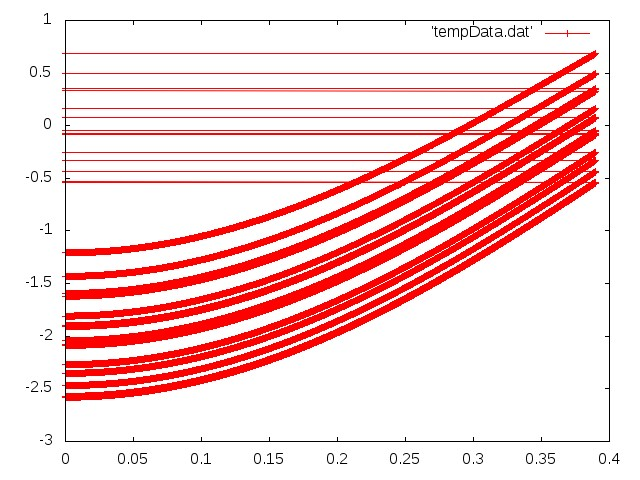
\includegraphics[width=0.3\textwidth]{harmonic1}
   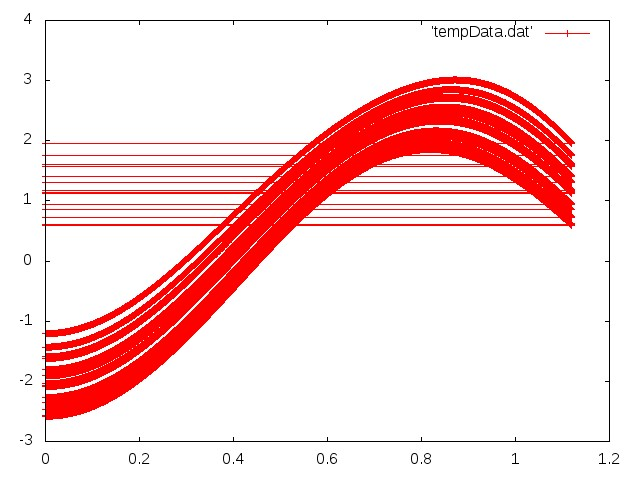
\includegraphics[width=0.3\textwidth]{harmonic2}
   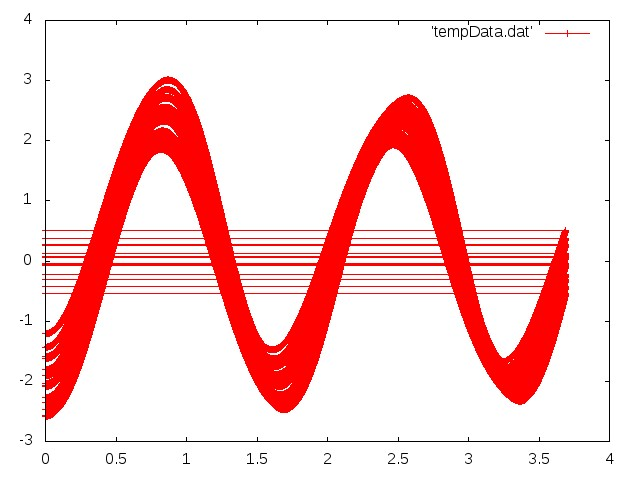
\includegraphics[width=0.3\textwidth]{harmonic} 
\end{center}
% }
% \end{figure}

\section*{Immediate Goals}
Numerically, extension to many particles and ability to handle spins are the essential next steps. These are required to validate the spin GHZ test as described. Theoretically, improvement of the phase space GHZ test is desired so that normalizable states can yield the paradox. The analogue of the SG apparatus for measuring $p$ is essential for a Bohmian analysis.
% }

% \blocknode
% {Future Scope}
% {
\section*{Future Scope}
A more ambitious goal would be to explore phase space contextuality \cite{AliContext} using BM to understand its relation with non locality more directly. A puzzling question is that while formally in QM, spins and (q,p) are handled rather similarly, why can't we extend BM in a manner such that spins are as `deterministic' as (q,p)? It is worth attempting to find such a formulation or to show that it doesn't exist. This is of great interest for this answer must depend on the fundamental difference between spins and (q,p) as properties. The thesis problem is a step in this direction.
}

\blocknode
{Acknowledgement and References}
{
\section*{Acknowledgement}
I thank my project guide Prof. Arvind for his timely guidance and encouragement, despite not having faith in Bohmian Mechanics. I am greatful to Dr. Abhishek Chowdhury and Dr. Sudeshna Sinha for their brief yet extremely useful assistance with the simulation. I also acknowledge my QCQI group members, Kishor Bharti, Rajendra Bhati and Jaskaran Singh for various discussions. The QCQI group meetings have been conducive in narrowing the thesis problem; the speakers Samridhi Gambhir and Arun Sehrawat deserve a special mention. 

%\nocite{*}
\tiny{
\bibliography{summary}}

}

%\bibliography{summary}


    % \coloredbox{colorthree!50!}{
    %   \textbackslash documentclass\{a0poster\}\\
    %   \textbackslash usepackage\{fancytikzposter\} \% here most of the things are
    %   defined \\

    %   \% change parameters only after this line\\

    %   \textbackslash usepackage{\small[margin=\textbackslash margin \ cm,
    %     paperwidth=84.1cm, paperheight=118.9cm]\{ geometry\}} \\

    %   \textbackslash title\{Title\}\\
    %   \textbackslash author\{Author\textbackslash\textbackslash
    %   Institution\textbackslash\textbackslash
    %   \textbackslash texttt\{email\}\}\\
    %   \textbackslash begin\{document\}\\
    %   \textbackslash AddToShipoutPicture\{\textbackslash BackgroundPicture\}\\


    %   \textbackslash noindent \\
    %   \textbackslash begin\{tikzpicture\} \\
    %   \textbackslash initializesizeandshifts \\

    %   \textbackslash titleblock\{50\}\{1\}\\
    %   \textbackslash blocknode\{Block Title\}\{Block Content\}\\
    %   \textbackslash startsecondcolumn\\
    %   \textbackslash blocknode\{Block Title 2\}\{Block Content 2\}\\
    %   \textbackslash end\{tikzpicture\}\\
    %   \textbackslash end\{document\}
    % }
  % }


  % %% a callout block
  % %% #1 - rotate angle (optional), #2 - from, #3 - where, #4 - width, #5 - text
  % %%%%%%%%%% ------------------------------------------ %%%%%%%%%%
  % \calloutblock{($(box.center)+(-2,-8)$)}
  % {($(box.center)+(10,-1)$)}
  % {19cm}
  % {\small
  %   Macro for creating a block node:
  %   \begin{itemize}
  %   \item[] \textbackslash blocknode\{Block Title\}\{Block Content\}
  %   \end{itemize}
  %   Macro \textbackslash blocknode has three parameters. The first one is
  %   optional and it is the position of the block. The first block will be
  %   automatically placed to (\$(firstrow)-(xshift)-(yshift)\$), which is the
  %   left corner below the title block. In most of the templates, (firstrow) is
  %   set to (title.south), where \emph{title} is the alias for the title
  %   block. Each subsequent block is automatically placed to
  %   [(\$(box.south)-(yshift)\$)], i.e., below the previous block aliased
  %   \emph{box}.  You can also use an explicit parameter, e.g., $(-10,30)$ (note
  %   that (0,0) is the center of the poster). The second parameter is the title
  %   of the block. Finally, the last parameter is the  actual content. 
  % }




 %  %% by default, the position of the new block node is right below the previous
 %  %% block node, stored in (currenty)
 %  %% box is the alias of the previous block, so we can refer to its boundaries

 %  %%%%%%%%%% ------------------------------------------ %%%%%%%%%%
 %  \blocknode{Making Title}%
 %  {To make title, use the standard commands \textbackslash title and
 %    \textbackslash author in the preamble, and then the following macro:
 %    \begin{itemize}
 %    \item[] \textbackslash titleblock\{50\}\{1.5\}
 %    \end{itemize}
 %    Macro \textbackslash titleblock has three parameters. The first one is
 %    optional and it specifies the shift of the title block w.r.t.\ its default
 %    position, which is set to (\$0.5*(0,\textbackslash
 %    paperheight)-(0,\textbackslash margin)\$). The second parameter is the width
 %    of the title block, and the third parameter is the scaling ratio (to make
 %    the title bigger or smaller).\\

 %    \small
 %    The syntax for specifying authors is similar to the one in aaai.sty.  Author
 %    information can be set in various styles: For several authors from the same
 %    institution:
 %    \begin{itemize}\item[] 
 %      \textbackslash author\{Author 1 \textbackslash and ... \textbackslash and
 %      Author n \textbackslash\textbackslash\\ 
 %      Address line \textbackslash\textbackslash \
 %      ... \textbackslash\textbackslash \ Address line\}
 %    \end{itemize}

 %    If the names do not fit well on one line use
 %    \begin{itemize}\item[] 
 %      \textbackslash author\{Author 1 \textbackslash\textbackslash \
 %      \{\textbackslash bf Author 2\} \textbackslash\textbackslash \
 %      ... \textbackslash\textbackslash \
 %      \{\textbackslash bf Author n\} \textbackslash\textbackslash\\
 %      Address line \textbackslash\textbackslash \
 %      ... \textbackslash\textbackslash \ Address line\}
 %    \end{itemize}

 %    For authors from different institutions: 
 %    \begin{itemize}\item[] 
 %      \textbackslash author\{Author 1 \textbackslash\textbackslash \ Address
 %      line \textbackslash\textbackslash \ ... \textbackslash\textbackslash \
 %      Address line \\ \textbackslash And ... \textbackslash And \\
 %      Author n \textbackslash\textbackslash \ Address line
 %      \textbackslash\textbackslash \ ... \textbackslash\textbackslash \ Address
 %      line\}
 %    \end{itemize}
    
 %    To start a separate ``row'' of authors use \textbackslash AND, as in
 %    \begin{itemize}\item[] 
 %      \textbackslash author\{Author 1 \textbackslash\textbackslash \ Address line
 %      \textbackslash\textbackslash \ ... \textbackslash\textbackslash \ Address
 %      line \textbackslash AND\\ Author 2 \textbackslash\textbackslash \ Address line
 %      \textbackslash\textbackslash \ ... \textbackslash\textbackslash \ Address
 %      line \textbackslash And\\ Author 3 \textbackslash\textbackslash \ Address line
 %      \textbackslash\textbackslash \ ... \textbackslash\textbackslash \ Address
 %      line\}
 %    \end{itemize}
 %    (though, I must say \textbackslash and ... \textbackslash and did not work for
 %    me with more than 2 authors, so just use commas where you need if it does
 %    not work for you either).
 %  }
  

 %  %%%%%%%%%% ------------------------------------------ %%%%%%%%%%
 %  \blocknodew[($(currenty)-(3.5,0)$)]{30}{Variable Width Block Nodes} %
 %  { You can also create blocks of arbitrary width
 %    \begin{itemize}
 %    \item[] \textbackslash blocknodew[coordinate]\{Block width\}\{Block Title\}%
 %      \{Block Content\}
 %    \end{itemize} 
 %    % 
 %    In this case it is better to specify coordinate manually if you want to have
 %    blocks aligned vertically. \\

 %    Note that (xshift) and (yshift) are coordinates created in macro
 %    \textbackslash initializesizeandshifts, and they allow to have relative
 %    positioning of block nodes in an automatic fashion. If you want to define
 %    your own shifts, set new values for (xshift) and (yshift) using commands
 %    \textbackslash setxshift and \textbackslash setyshift.\\

 %    Also, it might be useful to know the y-coordinate of the south border of the
 %    previous block. You can retrieve it by using the command
 %    \begin{itemize}
 %    \item[] \textbackslash getcurrentrow\{box\} or \textbackslash getcurrentrow\{note\}
 %    \end{itemize}
 %    This coordinate will be stored in (currentrow), which can be used to
 %    specify the location of the next block node.
 %  }


 %  %%%%%%%%%% ------------------------------------------ %%%%%%%%%%
 %  \plainblock[5]{($(currenty)+(4,2)$)}{35}{fancyTikZposter template} %
 %  {
    
 %    \vspace{0.3cm}
 %    It is a template for scientific posters based on a0poster and TikZ
 %    only. The current version contains five (plus one) different templates (see my
 %    posters
 %    % 
 %    \href{http://www.inf.unibz.it/~ebotoeva/presentations/abcrs-KR-12-poster.pdf}{%
 %      \underline{here}} and
 %    % 
 %    \href{http://www.inf.unibz.it/~ebotoeva/presentations/boto-RR-12-poster.pdf}{%
 %      \underline{here}}). The sources of this pdf file can be found
 %    \href{http://www.inf.unibz.it/~ebotoeva/tikz/tikzposter_sources.zip}{\underline{here}}.}

  


 %  %%%%%%%%%%%%% NEW COLUMN %%%%%%%%%%%%%%% 
 %  \startsecondcolumn 

 %  %%%%%%%%%% ------------------------------------------ %%%%%%%%%%
 %  \blocknode%
 %  {Block Nodes in the Second Column}%
 %  {To start the second column or the third column use commands
 %    \begin{itemize}
 %    \item[] \textbackslash startsecondcolumn, and \textbackslash startthirdcolumn.
 %    \end{itemize}
 %    If the number of columns is 2, then the last command will not have
 %    effect. \\

 %    You can also start a new column with an arbitrary x-coordinate by specifying
 %    explicitly the coordinate of the new block node as follows:
 %    \begin{itemize}
 %    \item[] \textbackslash blocknode[(\$(firstrow)-(yshift)+(x,0)\$)]\{Block
 %      Title\}\{Block Content\}
 %    \end{itemize}

 %    % 
 %  }


  
 %  %%%%%%%%%% ------------------------------------------ %%%%%%%%%%
 %  \blocknode{Useful Macro Within Block Nodes}%
 %  {There are three types of colored boxes/blocks that you can use inside block
 %    nodes to highlight information. \\
    
 %    \begin{tabular}[t]{ll}
 %      \begin{minipage}{0.5\linewidth}
 %        \innerblock{Theorem} {Statement}
 %      \end{minipage}
 %      & 
 %      \textbackslash innerblock\{Theorem\}\{Statement\}\\

 %      \begin{minipage}{0.5\linewidth}
 %        \innerblockplain[colorone!80!]{Text}
 %      \end{minipage}
 %      &
 %      \textbackslash innerblockplain[colorone!80!]\{Text\}\\ 

 %      \begin{minipage}{0.5\linewidth}
 %        \coloredbox{colorthree!50!}{Text}
 %      \end{minipage}
 %      &
 %      \textbackslash coloredbox\{colorthree!50!\}\{Text\}
 %    \end{tabular}

 %    \vspace{0.5cm}
 %    The default figure environment does not work within a tikzpicture. I created
 %    a new figure environment that can be used instead, based on the code sent by
 %    Stephan Thober.
 %    \begin{itemize}
 %    \item[] \textbackslash begin\{tikzfigure\}[Caption]\\
 %      \ldots\\
 %      \textbackslash end\{tikzfigure\}
 %    \end{itemize} 
 %    % 

 %    \begin{tikzfigure}[A shaded circle]
 %      \begin{tikzpicture}
 %        \draw[draw=none,inner color=colorthree, outer color=colorone] (0,0) circle (2cm);
 %      \end{tikzpicture}
 %    \end{tikzfigure}
 %  }


 %  %%%%%%%%%% ------------------------------------------ %%%%%%%%%%
 %  \calloutblock{($(box.south east)-(8,-2)$)}
 %  {($(box.south east)-(16,2)$)}
 %  {30cm}
 %  {
 %    There are also callout blocks that allow for a more interesting layout of the
 %    poster. 
 %    \begin{itemize}
 %    \item[] \textbackslash calloutblock[rotate angle]\{from
 %      coordinate\}\{coordinate\}\{Block Width\}\{Block Content\} 
 %    \end{itemize}
 %    The alias for such blocks is \emph{note}.
 %  }


 %  %% to place the next node centered vertically in the second column, we can
 %  %% obtain the y-coordinate of the previous node using macro
 %  %% \getcurrentrow{note}, where note is the alias of the callout node, and
 %  %% then specify the coordinate of the next node using coordinate (currentrow)
 %  \getcurrentrow{note}


 %  %% a plain block
 %  %% #1 - rotate angle (optional), #2 - where, #3 - width, #4 - title, #5 - text
 %  %%%%%%%%%% ------------------------------------------ %%%%%%%%%%
 %  \plainblock{($(currentrow)+(xshift)-(yshift)$)}%[($(currenty)+(0,10)$)]%
 %  {32}{Plain blocks} %
 %  {These blocks are similar to callout blocks. They allow for specifying the
 %    title of the block.
 %    \begin{itemize}
 %    \item[] \textbackslash plainblock[rotate angle]\{coordinate\}\{Block Width\}\{Block
 %      Title\}\{Block Content\} 
 %    \end{itemize}
 %  }


 
 %  %% the coordinate (currenty) is used in the default placing of the next blocknode
 % \getcurrentrow{note}
 % \coordinate (currenty) at ($(currentrow)+(xshift)-(yshift)$);



 %   %%%%%%%%%%%%% NEW COLUMN %%%%%%%%%%%%%%% 
 %  %% (if column number is 3)
 %  \startthirdcolumn

 %  %%%%%%%%%% ------------------------------------------ %%%%%%%%%%
 %  \blocknode {Personalizing the Poster}%
 %  {It is possible to adjust the layout of the poster. To impose your own
 %    setting, you can use these macros:
 %    \begin{itemize}
 %    \item Macros for changing sizes
 %      \begin{itemize}
 %      \item[] \textbackslash setmargin\{4\},
 %        %% the height of the head drawing on top
 %        %% applicable to templates N2 and 4
 %        \textbackslash setheaddrawingheight\{14\},
 %        %% the space between two or more groups of authors from different
 %        %% institutions
 %        %% used in \maketitle
 %        \textbackslash setinstituteshift\{10\},\\
 %        %% the space between the blocks
 %        %% default value is 2cm
 %        \textbackslash setblockspacing\{2\},
 %        %% the height of the title stripe in block nodes, decrease it to save space
 %        %% default value is 3cm
 %        \textbackslash setblocktitleheight\{3\}
 %      \end{itemize}

 %    \item Other structural macros
 %      \begin{itemize}
 %      \item[]  %% the number of columns in the poster, possible values 2,3
 %        %% default value is 2
 %        \textbackslash setcolumnnumber\{3\},
 %        %% which template to use 
 %        %% N1 simple, standard look, with a colored background and gray boxes
 %        %% N2 board with nodes
 %        %% N3 another standard look
 %        %% N4 envelope like look
 %        %% N5 with a wave-like head, original idea taken from
 %        %%%% http://fc09.deviantart.net/fs71/f/2010/322/1/1/scientific_poster_by_nabuy-d333ria.jpg
 %        %% N6 experimental, oriental style, largely based on template N3
 %        \textbackslash usetemplate\{6\},\\
 %        \textbackslash usecolortemplate\{4\},
 %        \textbackslash usebackgroundtemplate\{5\},
 %        \textbackslash usetitletemplate\{2\},\\
 %        \textbackslash useblocknodetemplate\{5\},
 %        \textbackslash useinnerblocktemplate\{3\},
 %        \textbackslash useplainblocktemplate\{4\}

 %      \end{itemize}

 %    \item Macro for adding logos to the title block
 %      \begin{itemize}
 %      \item[] \textbackslash addlogo[south west]\{(0,0)\}\{6cm\}\{filename\}
 %      \end{itemize}

 %    \item Macros for the basic colors
 %      \begin{itemize}
 %      \item[] \textbackslash setfirstcolor\{green!70!\}, % default 116699
 %        \textbackslash setsecondcolor\{gray!80!\}, % default CCCCCC
 %        \textbackslash setthirdcolor\{red!80!black\}% default 991111
 %      \end{itemize}

 %    \item Macros for specific colors:
 %      \begin{itemize}
 %      \item[] \textbackslash setbackgrounddarkcolor\{colorone!70!black\},
 %        \textbackslash setbackgroundlightcolor\{{\small colorone!70!}\},\\
 %        \textbackslash settitletextcolor\{textcolor\},
 %        \textbackslash settitlefillcolor\{white\},
 %        \textbackslash settitledrawcolor\{colortwo\},\\
 %        \textbackslash setblocktextcolor\{textcolor\},
 %        \textbackslash setblockfillcolor\{white\},\\
 %        \textbackslash setblocktitletextcolor\{colorone\},
 %        \textbackslash setblocktitlefillcolor\{colortwo\}, \\
 %        \textbackslash setplainblocktextcolor\{textcolor\},
 %        \textbackslash setplainblockfillcolor\{colorthree!40\},\\
 %        \textbackslash setplainblocktitletextcolor\{textcolor\},
 %        \textbackslash setplainblocktitlefillcolor\{colorthree!60\}, \\
 %        \textbackslash setinnerblocktextcolor\{textcolor\},
 %        \textbackslash setinnerblockfillcolor\{white\},\\
 %        \textbackslash setinnerblocktitletextcolor\{white\},
 %        \textbackslash setinnerblocktitlefillcolor\{colorthree\},
 %      \end{itemize}
 %    \end{itemize}
  % }



\end{tikzpicture}


\end{document}




